% !TEX TS-program = pdflatex
% !TEX encoding = UTF-8 Unicode

% This is a simple template for a LaTeX document using the "article" class.
% See "book", "report", "letter" for other types of document.

\documentclass[11pt]{article} % use larger type; default would be 10pt

\usepackage[utf8]{inputenc} % set input encoding (not needed with XeLaTeX)

%%% Examples of Article customizations
% These packages are optional, depending whether you want the features they provide.
% See the LaTeX Companion or other references for full information.

%%% PAGE DIMENSIONS
\usepackage{geometry} % to change the page dimensions
\geometry{a4paper} % or letterpaper (US) or a5paper or....
% \geometry{margin=2in} % for example, change the margins to 2 inches all round
% \geometry{landscape} % set up the page for landscape
%   read geometry.pdf for detailed page layout information

\usepackage{graphicx} % support the \includegraphics command and options
\usepackage[spanish]{babel}

% \usepackage[parfill]{parskip} % Activate to begin paragraphs with an empty line rather than an indent

%%% PACKAGES
\usepackage{booktabs} % for much better looking tables
\usepackage{array} % for better arrays (eg matrices) in maths
% \usepackage{paralist} % very flexible & customisable lists (eg. enumerate/itemize, etc.)
\usepackage{verbatim} % adds environment for commenting out blocks of text & for better verbatim
\usepackage{subfig} % make it possible to include more than one captioned figure/table in a single float
% These packages are all incorporated in the memoir class to one degree or another...
\usepackage{multicol}

\usepackage{graphicx}


%%% HEADERS & FOOTERS
\usepackage{fancyhdr} % This should be set AFTER setting up the page geometry
\pagestyle{fancy} % options: empty , plain , fancy
\renewcommand{\headrulewidth}{0pt} % customise the layout...
\lhead{}\chead{}\rhead{}
\lfoot{}\cfoot{\thepage}\rfoot{}

%%% SECTION TITLE APPEARANCE
\usepackage{sectsty}
\allsectionsfont{\sffamily\mdseries\upshape} % (See the fntguide.pdf for font help)
% (This matches ConTeXt defaults)

%%% ToC (table of contents) APPEARANCE
\usepackage[nottoc,notlof,notlot]{tocbibind} % Put the bibliography in the ToC
\usepackage[titles,subfigure]{tocloft} % Alter the style of the Table of Contents
\renewcommand{\cftsecfont}{\rmfamily\mdseries\upshape}
\renewcommand{\cftsecpagefont}{\rmfamily\mdseries\upshape} % No bold!

%%% END Article customizations

%%% The "real" document content comes below...

\title{Propuesta de Proyecto\\Problemas Especiales de Ingeniería en Computación}
\author{Jaime Castells\\Efraín Astudillo}
%\date{} % Activate to display a given date or no date (if empty),
         % otherwise the current date is printed 

\begin{document}
\maketitle

%\tableofcontents

\section{Introducción y Justificación}

La Realidad Virtual y Realidad Aumentada se encuentran cada vez más presentes en nuestras vidas cotidianas. 
La necesidad de desarrollo para estas herramientas se ha vuelto un factor muy importante para los estudiantes de ingeniería. 

La Realidad Aumentada interactúa con espacios físicos agregando información adicional a lo que se está viendo a través de una cámara web o cámara
del celular. La Realidad Virtual reemplaza el mundo real por uno totalmente virtual creado por el computador\cite{rvadefinition}. 
Los usuarios de estos sistemas deben poder interactuar con los objetos mostrados en pantalla usando dispositivos como el Kinect, Sensores de Movimiento, 
Guantes con sensores, Wii, Marcas Fiduciales, etc. Es importante analizar y considerar las Interfaces de Usuario que se podrían implementar en estos 
sistemas para brindar una buena experiencia al usuario. A través de este documento presentaremos algunas propuestas para ser realizadas como proyecto de la materia 
Problemas Especiales de Ingeniería en Computación.

\section{Propuestas}

\subsection {Interfaz gafas-pantalla}
\begin{itemize}
 \item Una interesante propuesta sería mostrar códigos en la pantalla táctil que las gafas 3D lo traduzcan a animaciones, y que la persona usando las gafas 
  pueda verlas. Esta persona puede escoger qué códigos mostrar en pantalla, agrandarlos, y juntar muchos a la vez. Lo interesante de aquí es que las animaciones, 
  al estar juntas una de otra, pueden interactuar entre ellas y mostrar resultados diferentes.
  \item Otra propuesta podría ser una Pizarra Interactiva e implementar un juego de Tic Tac Toe utilizando Realidad Aumentada y el Leap Motion como dispositivo 
  de entrada con el que el usuario podrá interactuar como se puede apreciar en la Figura \ref{imgLeap}.
  
  \begin{figure}
   \centerline{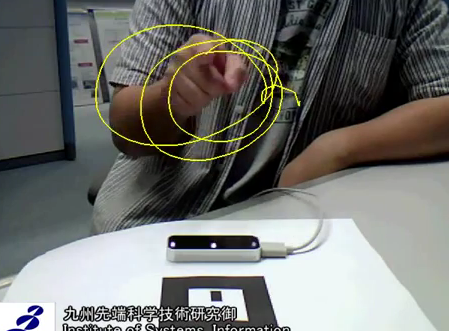
\includegraphics[scale=0.50]{./img/leapAugmented.png}}
   \caption{Pizarra Interactiva con Realidad Aumentada}
   \label{imgLeap}
  \end{figure}
  
  \begin{figure}
   \centerline{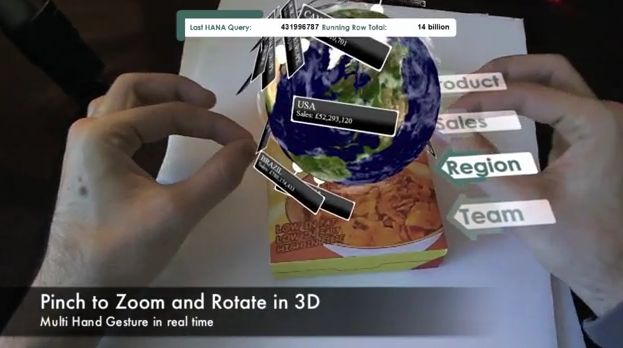
\includegraphics[scale=0.40]{./img/kinectAugmented.png}}
   \caption{Ejemplo de Sistema de Navegación utilizando Realidad Aumentada y el Kinect}
   \label{imgKinect}
  \end{figure}
  \item También se podría implementar un Sistema de Navegación de un Cráneo Interactivo como soporte educativo para el aprendizaje de las diferentes partes del Cráneo 
  Humano utilizando Kinect y Realidad Aumentada. El Kinect se lo usa en un API llamado \emph{Finger-precise hand-tracking (http://www.threegear.com/)} y nos permitirá obtener los gestos realizados 
  por las manos. Un ejemplo similar se pueden apreciar en la Figura \ref{imgKinect}.
  


\end{itemize}


\section{Herramientas a Usarse}

\begin{itemize}
 \item \textbf{Pantalla táctil:}
 Una de las herramientas puede ser la pantalla tácil, de 42 pulgadas, que puede mostrar cualquier gráfico que querramos. Se puede armar una interfaz táctil para el usuario 
  y que éste interactúe con la pantalla.
  \item \textbf{Gafas 3D:}
  Las gafas 3D pueden ser utilizadas y mostrar algún gráfico al frente de la persona, dado que contienen cámaras en la parte ocular.
  \item \textbf{Kinect:}
  El dispositivo Kinect desarrollado por Microsoft puede ser utilizado para detectar gestos o comandos realizados por las manos o extremidades.
  \item \textbf{Leap Motion:}
  El Leap Motion es un dispositivo que detecta gestos realizados con las manos con gran precisión.
\end{itemize}




\begin{thebibliography}{9}
 \bibitem{lamport94}
 Leslie Lamport, \emph{\LaTeX: A Document Preparation System}
 
 \bibitem{rvadefinition}
 Montiel, Alejandro Gael. Realidad Aumentada y Realidad Virtual: ¿Cuál es la diferencia?. \emph{Interactive Magazine} [en línea]. 23 de Abril de 2013.
 [fecha de consulta: 19 de Octubre de 2013]. Disponible en: http://revistainteractive.com/realidad-aumentada-y-realidad-virtua/
\end{thebibliography}

\end{document}
